Zun\"achst ist es vonn\"oten zu entscheiden, wann das Normalenb\"undel \(\nu\) einer in eine eingebetteten Sph\"are nicht nur stabil trivial, sondern bereits trivial ist. Da \(\nu\) stabil trivial ist, liegt es in \(\ker S_*\). Betrachte hierzu zun\"achst die Abbildung
\[\Phi\colon\ker S_*\to\mathbb{Z}\,,\eqcl{\xi}\mapsto\left\langle e\left(\xi\right),\eqcl{\mathbb{S}^k}\right\rangle\,.\]
Aus den Eigenschaften der Euler-Klasse folgt, dass dies ein wohldefinierter Homomorphismus ist. Dieser ist jedoch f\"ur ungerade \(k\) trivial, da in diesem Fall \(\ker S_*\cong\mathbb{Z}_2\) endlich ist.
\begin{lemma}\label{lem:phi_mono_even}
    F\"ur gerade \(k\) ist \(\Phi\) ein Monomorphismus, der lediglich gerade Werte annimmt.
\end{lemma}
\begin{proof}
    Der Kern \(\ker S_*\) wird von \(\eqcl{\tau_k}\) erzeugt, und ist, da \(k\) gerade ist, zyklisch unendlich. Folglich ist jedes \(\eqcl{\xi}\in\ker S_*\) ein Vielfaches von \(\eqcl{\tau_k}\), sei etwa \({\eqcl{\xi}=\beta\cdot\eqcl{\tau_k}}\). Da die Euler-Klasse von \(\tau_k\) das Doppelte eines Erzeugers \(g\in H^k(\mathbb{S}^k)\) ist (Siehe \cite{hatcher2017vector} Proposition 3.14), gilt
    \[\Phi(\eqcl{\xi})=\left\langle e(\xi),\eqcl{\mathbb{S}^k}\right\rangle=2\beta\cdot\left\langle g,\eqcl{\mathbb{S}^k}\right\rangle\,.\]
    Da \(\langle g,\eqcl{\mathbb{S}^k}\rangle\not=0\) ist, ist dies genau dann null, wenn \(\beta=0\), und somit \(\eqcl{\xi}=0\) ist.
\end{proof}
Sei \(\mathcal{M}^{2k}\) eine \(\pi\)-Mannigfaltigkeit, und \(\mathcal{S}^k\hookrightarrow\mathring{\mathcal{M}}\) eine eingebettete Sph\"are. Dann folgt aus dem vorangegangenen Lemma, dass das Normalenb\"undel \(\nu\) von \(\mathcal{S}\) genau dann trivial ist, wenn \(\Phi(\nu)=0\) gilt. Um dies zu entscheiden ist das folgende Lemma hilfreich.
\begin{lemma}\label{lem:euler_dual}
    Sei \(\mathcal{M}^{i+j}\) eine orientierte Mannigfaltigkeit und \(\iota\colon\mathcal{V}^i\hookrightarrow\mathring{\mathcal{M}}\) eine geschlossene Untermannigfaltigkeit mit Normalenb\"undel \(\nu\). Dann gilt
    \begin{equation}\label{eq:euler_dual}
        e(\nu)=\pm\iota^*q^*\eqcl{\mathcal{V}\mathrel{|}\mathcal{M}}^*\quad\text{also}\quad\langle e(\nu),\eqcl{\mathcal{V}}\rangle=\pm\eqcl{\mathcal{V}\mathrel{|}\mathcal{M}}\cdot\eqcl{\mathcal{V}\mathrel{|}\mathcal{M}}\,.
    \end{equation}
\end{lemma}
\begin{proof}
    Sei \(\mathcal{D}\subseteq\mathring{\mathcal{M}}\) eine geschlossene Tubenumgebung von \(\mathcal{V}\). Betrachte die kanonischen Inklusionen
    \[d\colon(\mathcal{D},\partial\mathcal{D})\hookrightarrow\big(\mathcal{M},\mathcal{M}\setminus\mathring{\mathcal{D}}\big)\quad\text{und}\quad f\colon(\mathcal{M},\partial\mathcal{M})\hookrightarrow\big(\mathcal{M},\mathcal{M}\setminus\mathring{\mathcal{D}}\big)\,.\]
    Sei \(X:=f_*\eqcl{\mathcal{M}}=d_*\eqcl{\mathcal{D}}\). Dann kommutiert das Diagramm
    \begin{center}
        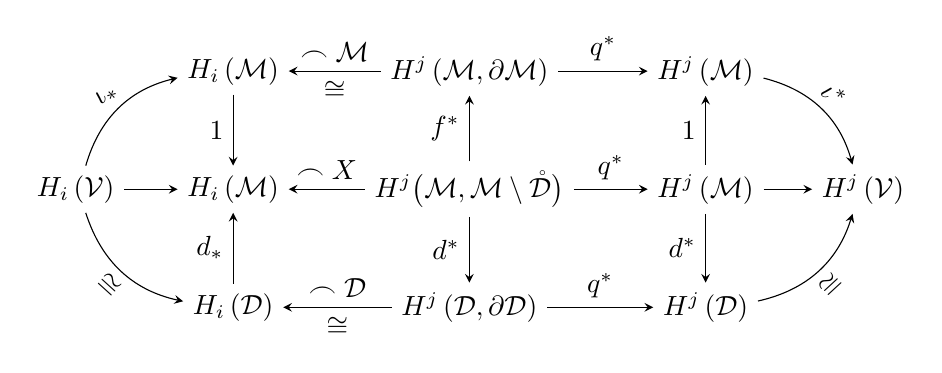
\begin{tikzpicture}
            \draw
                (0, 0) node (A) {\(H_i\left(\mathcal{V}\right)\)}
                (2, -1.5) node (B) {\(H_i\left(\mathcal{D}\right)\)}
                (2, 0) node (C) {\(H_i\left(\mathcal{M}\right)\)}
                (2, 1.5) node (D) {\(H_i\left(\mathcal{M}\right)\)}
                (5, -1.5) node (E) {\(H^j\left(\mathcal{D},\partial\mathcal{D}\right)\)}
                (5, 0) node (F) {\(H^j\big(\mathcal{M},\mathcal{M}\setminus\mathring{\mathcal{D}}\big)\)}
                (5, 1.5) node (G) {\(H^j\left(\mathcal{M},\partial\mathcal{M}\right)\)}
                (8, -1.5) node (H) {\(H^j\left(\mathcal{D}\right)\)}
                (8, 0) node (I) {\(H^j\left(\mathcal{M}\right)\)}
                (8, 1.5) node (J) {\(H^j\left(\mathcal{M}\right)\)}
                (10, 0) node (K) {\(H^j\left(\mathcal{V}\right)\)}

                (A) edge [-stealth, bend right] node [sloped, below] {\(\cong\)} (B)
                (A) edge [-stealth] (C)
                (A) edge [-stealth, bend left] node [sloped, above] {\(\iota_*\)} (D)
                
                (E) edge [-stealth] node [below] {\(\cong\)} node [above] {\(\frown\eqcl{\mathcal{D}}\)} (B)
                (E) edge [-stealth] node [above] {\(q^*\)} (H)
                (H) edge [-stealth, bend right] node [sloped, below] {\(\cong\)} (K)
                
                (F) edge [-stealth] node [above] {\(\frown X\)} (C)
                (F) edge [-stealth] node [above] {\(q^*\)} (I)
                (I) edge [-stealth] (K)

                (G) edge [-stealth] node [below] {\(\cong\)} node [above] {\(\frown\eqcl{\mathcal{M}}\)} (D)
                (G) edge [-stealth] node [above] {\(q^*\)} (J)
                (J) edge [-stealth, bend left] node [sloped, above] {\(\iota^*\)}  (K)
                
                (B) edge [-stealth] node [left] {\(d_*\)} (C)
                (D) edge [-stealth] node [left] {\(\mathbbm{1}\)} (C)
                
                (F) edge [-stealth] node [left] {\(d^*\)} (E)
                (F) edge [-stealth] node [left] {\(f^*\)} (G)
                
                (I) edge [-stealth] node [left] {\(d^*\)} (H)
                (I) edge [-stealth] node [left] {\(\mathbbm{1}\)} (J)
                ;
        \end{tikzpicture}
    \end{center}
    Hierbei korrespondiert ein Generator von \(H^j\left(\mathcal{D},\partial\mathcal{D}\right)\) mit der Thom-Klasse von \(\nu\), und wird deshalb in \(H^j(\mathcal{V})\) auf die Euler-Klasse von \(\nu\) abgebildet. Durch eine Jagd der Fundamentalklasse \(\eqcl{\mathcal{V}}\in H_i(\mathcal{V})\) durch die obere und untere Zeile ergibt sich
    \[\pm\iota^*q^*\eqcl{\mathcal{V}\mathrel{|}\mathcal{M}}^*=e(\nu)\,.\]
    Es gilt also
    \begin{align*}
        \mp\left\langle e(\nu),\eqcl{\mathcal{S}}\right\rangle&=\left\langle\iota^*q^*\eqcl{\mathcal{S}\mathrel{|}\mathcal{M}}^*,\eqcl{\mathcal{S}}\right\rangle\\
        &=\left\langle q^*\eqcl{\mathcal{S}\mathrel{|}\mathcal{M}}^*,\eqcl{\mathcal{S}\mathrel{|}\mathcal{M}}\right\rangle\mathop{=}^{\text{\tiny\eqref{eq:intersect_prop_2}}}\eqcl{\mathcal{S}\mathrel{|}\mathcal{M}}\cdot\eqcl{\mathcal{S}\mathrel{|}\mathcal{M}}\,.
    \end{align*}
\end{proof}
Der Beweis orientiert sich an einem \"ahnlichen Lemma aus Lecture 11 von \cite{auroux2012algebraic}.

\begin{theorem}\label{thm:intersect_even}
    Sei \(k\geq3\) gerade und \(\mathcal{M}^{2k}\) eine \((k-1)\)-zusammenh\"angende \(\pi\)-Mannig\-faltig\-keit. Dann ist die Schnittpaarung gerade, und es gilt \({x\cdot x=0}\) genau dann, wenn \({\alpha(x)=0}\) ist.
\end{theorem}
\begin{proof}
    Zun\"achst gilt \(\alpha(x)\in\ker S_*\) gem\"a\ss{} Gleichung \ref{eq:alpha_kernel}. Sei \({\iota\colon\mathcal{S}\hookrightarrow\mathring{\mathcal{M}}}\) eine \(x\) repr\"asentierende Einbettung mit Normalenb\"undel \(\nu\). Dann gelten per Definitionem
    \(x=\eqcl{\mathcal{S}\mathrel{|}\mathcal{M}}\) und \(\alpha(x)=\eqcl{\nu}\). Zusammen ergibt dies
    \[x\cdot x=\eqcl{\mathcal{S}\mathrel{|}\mathcal{M}}\cdot\eqcl{\mathcal{S}\mathrel{|}\mathcal{M}}\mathop{=}^{\text{\tiny\eqref{eq:euler_dual}}}\mp\left\langle e(\nu),\eqcl{\mathcal{S}}\right\rangle=\mp\Phi(\alpha(x))\,.\]
    Dann ist die Aussage des Satzes eine direkte Konsequenz von Lemma \ref{lem:phi_mono_even}.
\end{proof}
